% vim: set spell spelllang=en tw=100 et sw=4 sts=4 foldmethod=marker foldmarker={{{,}}} :

\documentclass[aspectratio=169,compress,10pt]{beamer}

\usepackage{tikz}
\usepackage{xcolor}
\usepackage{complexity}
\usepackage{hyperref}
\usepackage{microtype}
\usepackage{amsmath}                   % \operatorname
\usepackage{amsfonts}                  % \mathcal
\usepackage{amssymb}                   % \nexists
\usepackage[vlined]{algorithm2e} % algorithms
\usepackage{centernot}
\usepackage{listings}
\usepackage{csquotes}
\usepackage{fancyvrb}
\usepackage{bussproofs}
\usepackage{multicol}
\usepackage{booktabs}
\usepackage{mathtools}
\usepackage{pifont}
\usepackage{marvosym}
\usepackage{cancel}

\usefonttheme{professionalfonts}

\usetikzlibrary{shapes, arrows, shadows, calc, positioning, fit}
\usetikzlibrary{decorations.pathreplacing, decorations.pathmorphing, shapes.misc}
\usetikzlibrary{tikzmark, backgrounds}
\usetikzlibrary{trees, overlay-beamer-styles}

\tikzset{processarrow/.style={->, very thick, decorate, decoration={snake, post length=0.5mm}}}
\tikzset{brace/.style={decorate, decoration={brace}, very thick}}

\definecolor{uofguniversityblue}{rgb}{0, 0.219608, 0.396078}
\definecolor{uofgheather}{rgb}{0.356863, 0.32549, 0.490196}
\definecolor{uofgaquamarine}{rgb}{0.603922, 0.72549, 0.678431}
\definecolor{uofgslate}{rgb}{0.309804, 0.34902, 0.380392}
\definecolor{uofgrose}{rgb}{0.823529, 0.470588, 0.709804}
\definecolor{uofgmocha}{rgb}{0.709804, 0.564706, 0.47451}
\definecolor{uofgsandstone}{rgb}{0.321569, 0.278431, 0.231373}
\definecolor{uofgforest}{rgb}{0, 0.2, 0.129412}
\definecolor{uofglawn}{rgb}{0.517647, 0.741176, 0}
\definecolor{uofgcobalt}{rgb}{0, 0.615686, 0.92549}
\definecolor{uofgturquoise}{rgb}{0, 0.709804, 0.819608}
\definecolor{uofgsunshine}{rgb}{1.0, 0.862745, 0.211765}
\definecolor{uofgpumpkin}{rgb}{1.0, 0.72549, 0.282353}
\definecolor{uofgthistle}{rgb}{0.584314, 0.070588, 0.447059}
\definecolor{uofgrust}{rgb}{0.603922, 0.227451, 0.023529}
\definecolor{uofgburgundy}{rgb}{0.490196, 0.133333, 0.223529}
\definecolor{uofgpillarbox}{rgb}{0.701961, 0.047059, 0}
\definecolor{uofglavendar}{rgb}{0.356863, 0.301961, 0.580392}

% {{{ theme things
\useoutertheme[footline=authortitle]{miniframes}
\useinnertheme{rectangles}

\setbeamerfont{block title}{size={}}
\setbeamerfont{title}{size=\large,series=\bfseries}
\setbeamerfont{section title}{size=\large,series=\mdseries}
\setbeamerfont{author}{size=\normalsize,series=\mdseries}
\setbeamercolor*{structure}{fg=uofguniversityblue}
\setbeamercolor*{palette primary}{use=structure,fg=black,bg=white}
\setbeamercolor*{palette secondary}{use=structure,fg=white,bg=uofgcobalt}
\setbeamercolor*{palette tertiary}{use=structure,fg=white,bg=uofguniversityblue}
\setbeamercolor*{palette quaternary}{fg=white,bg=black}
\setbeamercolor{block body}{bg=structure!10}
\setbeamercolor{block title}{bg=structure,fg=white}
\setbeamertemplate{blocks}[rounded]
\setbeamercolor*{titlelike}{parent=palette primary}

\beamertemplatenavigationsymbolsempty

\setbeamertemplate{title page}
{
    \begin{tikzpicture}[remember picture, overlay]
        \node at (current page.north west) {
            \begin{tikzpicture}[remember picture, overlay]
                \fill [fill=uofguniversityblue, anchor=north west] (0, 0) rectangle (\paperwidth, -2.6cm);
            \end{tikzpicture}
        };

        \node (logo) [anchor=north east, shift={(-0.8cm,-0.2cm)}] at (current page.north east) {
            
\includegraphics[keepaspectratio=true,scale=0.5]{../../images/UoG_keyline.pdf}
        };

        \node (logo2) [anchor=north, below=0.2cm of logo.south] {
            
\includegraphics[keepaspectratio=true,scale=0.1]{../../images/RAEngWhite.pdf}
        };

        \coordinate (logos) at ($(logo.south)!0.5!(logo2.north)$);

        \node [anchor=west, xshift=0.8cm] at (current page.west |- logos) {
            \begin{minipage}{0.65\paperwidth}\raggedright
                {\usebeamerfont{title}\usebeamercolor[white]{}\inserttitle}\\[0.1cm]
                {\usebeamerfont{author}\usebeamercolor[white]{}\insertauthor}\\[0.1cm]
                {\usebeamerfont{author}\usebeamercolor[white]{}In collaboration with Emir
                Demirovi\'c, Matthew McIlree, Jakob Nordstr\"om, Andy Oertel, and Konstantin
                Sidorov}
            \end{minipage}
        };
    \end{tikzpicture}
}

\setbeamertemplate{section page}
{
    \begin{centering}
        \begin{beamercolorbox}[sep=12pt,center]{part title}
            \usebeamerfont{section title}\insertsection\par
        \end{beamercolorbox}
    \end{centering}
}

\newcommand{\frameofframes}{/}
\newcommand{\setframeofframes}[1]{\renewcommand{\frameofframes}{#1}}

\makeatletter
\setbeamertemplate{footline}
{%
    \begin{beamercolorbox}[colsep=1.5pt]{upper separation line foot}
    \end{beamercolorbox}
    \begin{beamercolorbox}[ht=2.5ex,dp=1.125ex,%
        leftskip=.3cm,rightskip=.3cm plus1fil]{author in head/foot}%
        \leavevmode{\usebeamerfont{author in head/foot}\insertshortauthor}%
        \hfill%
        {\usebeamerfont{institute in head/foot}\usebeamercolor[fg]{institute in head/foot}\insertshortinstitute}%
    \end{beamercolorbox}%
    \begin{beamercolorbox}[ht=2.5ex,dp=1.125ex,%
        leftskip=.3cm,rightskip=.3cm plus1fil]{title in head/foot}%
        {\usebeamerfont{title in head/foot}\insertshorttitle}%
        \hfill%
        {\usebeamerfont{frame number}\usebeamercolor[fg]{frame number}\insertframenumber~\frameofframes~\inserttotalframenumber}
    \end{beamercolorbox}%
    \begin{beamercolorbox}[colsep=1.5pt]{lower separation line foot}
    \end{beamercolorbox}
}

\makeatletter
\setbeamertemplate{mini frame}
{%
  \begin{pgfpicture}{0pt}{0pt}{.04cm}{.04cm}
    \pgfpathcircle{\pgfpoint{0.04cm}{0.04cm}}{0.04cm}
    \pgfusepath{fill,stroke}
  \end{pgfpicture}%
}
\setbeamertemplate{mini frame in current subsection}
{%
  \begin{pgfpicture}{0pt}{0pt}{.04cm}{.04cm}
    \pgfpathcircle{\pgfpoint{0.04cm}{0.04cm}}{0.04cm}
    \pgfsetfillcolor{section in head/foot.bg}
    \pgfusepath{fill,stroke}
  \end{pgfpicture}%
}

\setbeamersize{mini frame size=0.10cm, mini frame offset=0.06cm}
\makeatother

% }}}

\author{Ciaran McCreesh}
\title{Proof Logging for Dynamic Programming Algorithms}

\begin{document}

{
    \usebackgroundtemplate{
        \tikz[overlay, remember picture]
        \node[at=(current page.south), anchor=south, inner sep=0pt, yshift=-1.4cm]{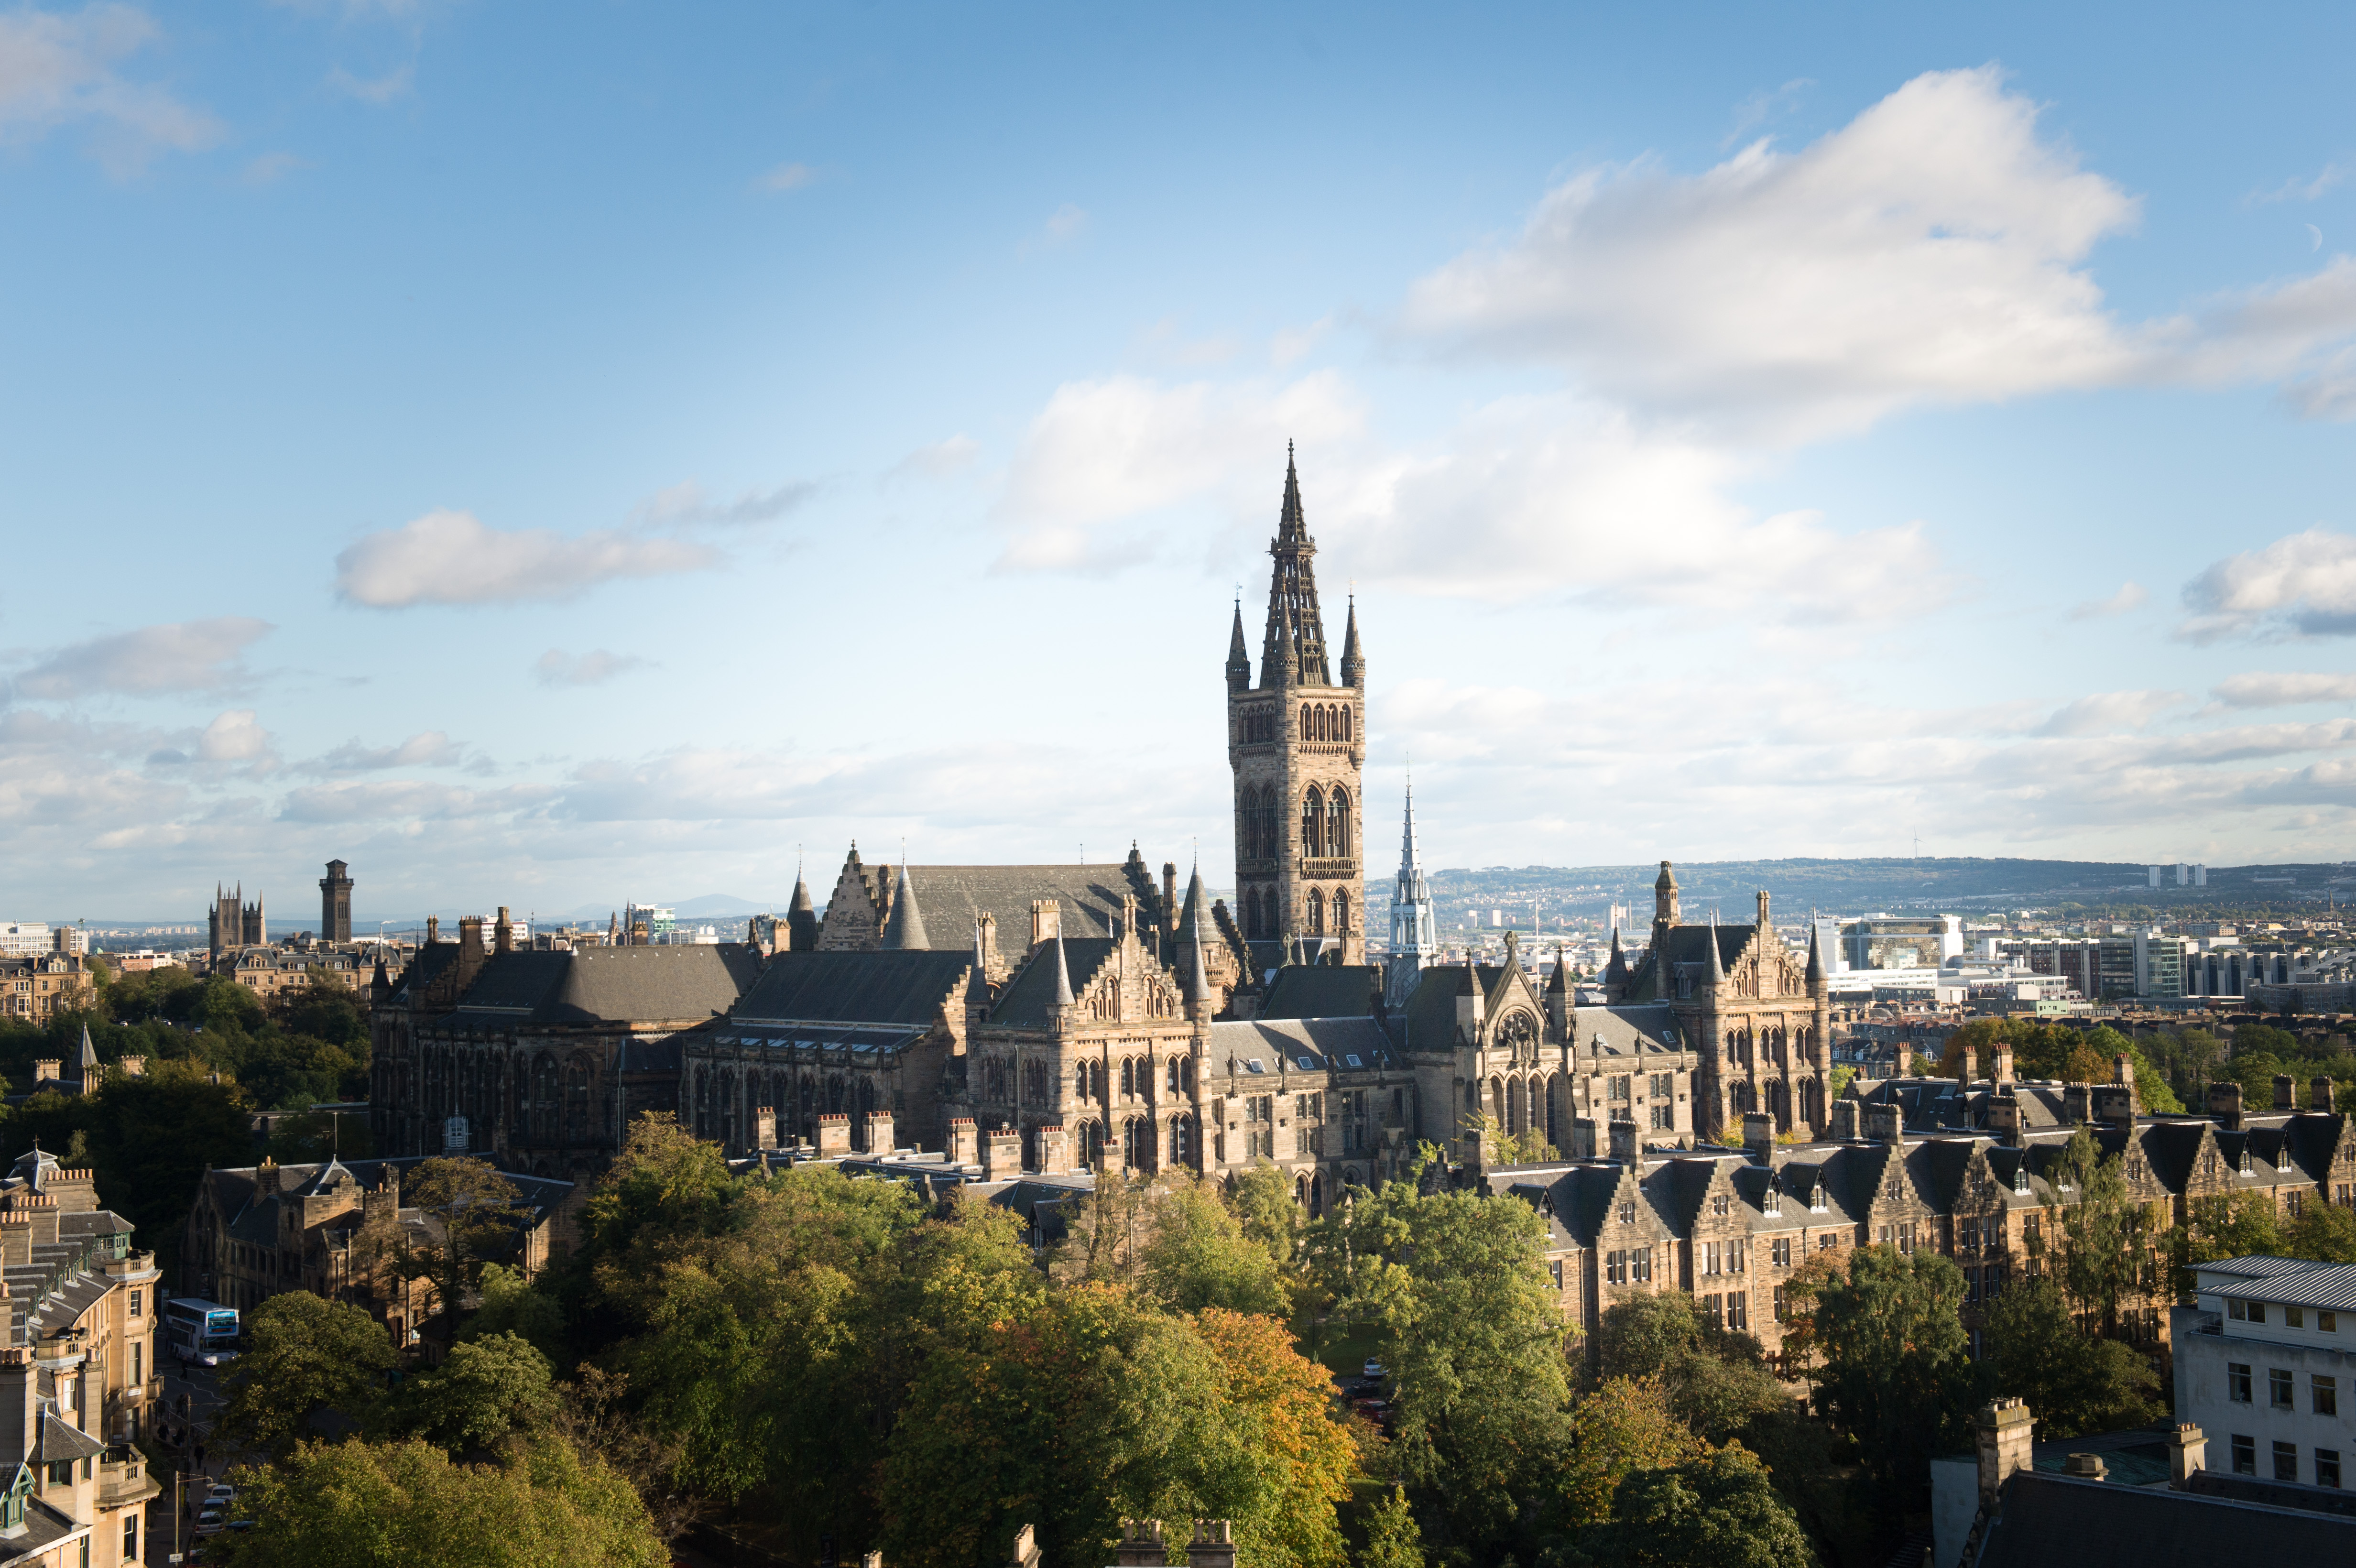
\includegraphics[keepaspectratio=true, width=\paperwidth]{../../images/background.jpg}};
    }
    \begin{frame}[plain,noframenumbering]
        \titlepage
    \end{frame}
}

\section{Knapsack}

\begin{frame}{Knapsack Problems}
\end{frame}

\begin{frame}{Dynamic Programming for Knapsack}
\end{frame}

\begin{frame}{Viewing Dynamic Programming as a Decision Diagram}
\end{frame}

\begin{frame}{Merging More States}
\end{frame}

\begin{frame}{Is It Correct?}
\end{frame}

\section{Proofs}

\begin{frame}{Proof Logging}
    \vspace*{-1.0em}
    \begin{center}
        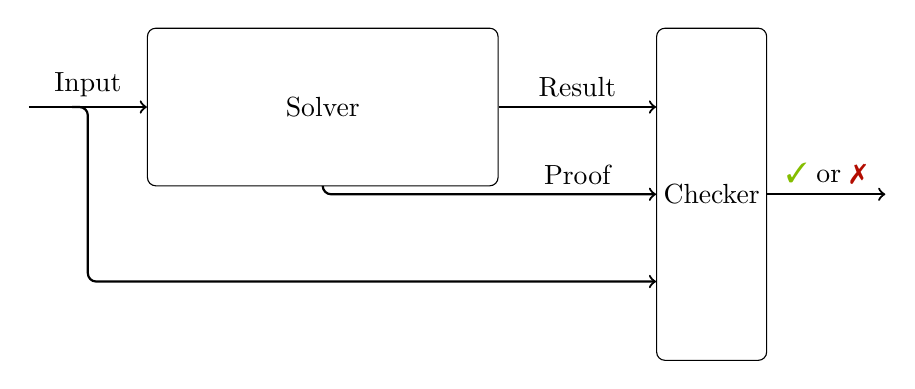
\begin{tikzpicture}
            \node (solver) [%
            inner xsep=5em,
            inner ysep=2.5em, 
            draw, rounded corners=3pt] { Solver };

            \node (checker) [%
            right=2cm of solver.north east, 
            anchor=north west,
            inner xsep=0.25em,
            draw, rounded corners=3pt, 
            minimum height=12em, 
            visible on=<3->] { Checker };

            \draw [->, thick] (solver.east) -- (solver.east -| checker.west)
                coordinate [midway] (solutionmid) node [above, midway]
                { 
                  Result
                };

            \draw [->, thick, rounded corners=3pt, visible on=<2->] (solver.south) -- (solver.south |- checker.west)
                -- (checker.west) coordinate [midway] (proofmid);

            \coordinate (prooflabel) at (proofmid-|solutionmid);
            \node [above=0cm of prooflabel, visible on=<2->] { Proof };

            \coordinate [right=1.5cm of checker.east] (verified);
            \draw [->, thick, visible on=<4->] (checker.east) -- (verified) node [above, midway] { \textcolor{uofglawn}{\ding{51}} or \textcolor{uofgpillarbox}{\ding{55}} };

            \coordinate [left=1.5cm of solver.west] (input);
            \draw [->, thick] (input) -- (solver.west) coordinate [midway] (inputmid) node [above, midway] { Input };

            \coordinate (checkerbotleft) at ($(checker.west)+($(checker.west)-(solver.east-|checker.west)$)$);

            \draw [->, thick, rounded corners=3pt, visible on=<3->] ($(inputmid)+(-0.2,0)$) -- (inputmid) -- (inputmid |- checkerbotleft) -- (checkerbotleft);
        \end{tikzpicture}
      \end{center}
    \vspace*{-0.7em}
  \begin{enumerate}
  \item<1->
    Run solver on problem input.
  \item<2->
    Get both a solution and a proof as output.
  \item<3->
    Feed input + solution + proof to proof checker.
  \item<4->
    Verify that proof checker says solution is correct.
  \end{enumerate}
\end{frame}

\begin{frame}{Pseudo-Boolean Problems}

    ?? negation of literals and constraints, normal form
\end{frame}

\begin{frame}{Knapsack as a Pseudo-Boolean Problem}
\end{frame}

\begin{frame}{Implications as Pseudo-Boolean Constraints}
\end{frame}

\begin{frame}{The VeriPB Proof System}
\end{frame}

\begin{frame}{Cutting Planes Proofs}
    \begin{minipage}[c]{0.35\framewidth}
        \textcolor{uofgcobalt}{\textbf{Model axioms}}
    \end{minipage}\hfill\begin{minipage}[c]{0.60\framewidth}
        \centering From the input
    \end{minipage}\medskip

    \begin{minipage}[c]{0.35\framewidth}
        \textcolor{uofgcobalt}{\textbf{Literal axioms}}
    \end{minipage}\hfill\begin{minipage}[c]{0.60\framewidth}\begin{prooftree}
        \AxiomC{~}
        \UnaryInfC{$\ell_i \ge 0$}
    \end{prooftree}\end{minipage}\medskip

    \begin{minipage}[c]{0.35\framewidth}
        \textcolor{uofgcobalt}{\textbf{Addition}}
    \end{minipage}\hfill\begin{minipage}[c]{0.60\framewidth}\begin{prooftree}
        \AxiomC{$\sum_i a_i \ell_i \ge A$}
        \AxiomC{$\sum_i b_i \ell_i \ge B$}
        \BinaryInfC{$\sum_i (a_i + b_i) \ell_i \ge A + B$}
    \end{prooftree}\end{minipage}\medskip

    \begin{minipage}[c]{0.35\framewidth}
        \textcolor{uofgcobalt}{\textbf{Multiplication}}\\
        for any $c \in \mathbb{N^+}$
    \end{minipage}\hfill\begin{minipage}[c]{0.60\framewidth}\begin{prooftree}
        \AxiomC{$\sum_i a_i \ell_i \ge A$}
        \UnaryInfC{$\sum_i { c a_i \ell_i } \ge c A$}
    \end{prooftree}\end{minipage}\medskip

    \begin{minipage}[c]{0.35\framewidth}
        \textcolor{uofgcobalt}{\textbf{Division}}\\
        for any $c \in \mathbb{N^+}$
    \end{minipage}\hfill\begin{minipage}[c]{0.60\framewidth}\begin{prooftree}
        \AxiomC{$\sum_i a_i \ell_i \ge A$}
        \UnaryInfC{$\sum_i {\left\lceil \frac{a_i}{c} \right\rceil} \ell_i \ge \left\lceil \frac{A}{c} \right\rceil$}
    \end{prooftree}\end{minipage}\medskip

    \begin{minipage}[c]{0.35\framewidth}
        \textcolor{uofgcobalt}{\textbf{Saturation}}
    \end{minipage}\hfill\begin{minipage}[c]{0.60\framewidth}\begin{prooftree}
        \AxiomC{$\sum_i a_i \ell_i \ge A$}
        \UnaryInfC{$\sum_i \operatorname{min}\left(a_i, A\right) \ell_i \ge A$}
    \end{prooftree}\end{minipage}
\end{frame}

\begin{frame}{CNF and Resolution}
\end{frame}

\begin{frame}{Reverse Unit Propagation}
\end{frame}

\begin{frame}{The Extension Rule}
  Suppose we want new, fresh variable
  $a$ encoding
  \begin{equation*}
        a
        \Leftrightarrow
        ( 3x + 2y + z + w \ge 3 )
  \end{equation*}

  Introduce constraints
    \begin{equation*}
    a \Rightarrow 3x + 2y + z + w \ge 3
    \qquad
        \overline{a} \Rightarrow
    3 \overline{x} + 2 \overline{y}  + \overline{z} + \overline{w} \ge 5
    \end{equation*}
    i.e.
  \begin{equation*}
    3 \overline{a} + 3x + 2y + z + w \ge 3
    \qquad
    5 a +
    3 \overline{x} + 2 \overline{y}  + \overline{z} + \overline{w} \ge 5
  \end{equation*}

  Should be fine, so long as $a$ hasn't been used before.
\end{frame}

\begin{frame}{Proofs Under Implication}
    \begin{theorem}
    Let's say we have a collection of constraints $\mathcal{C}$ and know how to get a proof deriving
        $D$. \\\medskip

    Suppose now we replace one or more constraints $C_i$ from $\mathcal{C}$ with implications $\land
        G_i \Rightarrow C$. \\\medskip

    Then we know how to get a proof deriving $\land \cup_i G_i \Rightarrow D$.
    \end{theorem}
    \begin{proof}[Handwavy proof sketch]
        For RUP, add in the implications and it ``just works''. \\\medskip

        For cutting planes, run the same proof, but saturate between each step. Use literal
        axioms at the end to re-introduce any assumptions that disappear from $\land \cup_i G_i$,
        and to fix up coefficients. \\\medskip

        For extension rules, keep them as-is.
    \end{proof}
\end{frame}

\begin{frame}{Proofs for Backtracking Search}
\end{frame}

\begin{frame}{Proofs for Dynamic Programming Algorithms for Knapsack}
\end{frame}

\begin{frame}{Extension Variables for States}
    For each state (or entry in the matrix) on layer $\ell$, define
    \begin{align*}
        W^{\ell}_{w} &\Leftrightarrow \sum_{i=1}^{\ell} W_i x_i \ge w \\[0.3cm]
        P^{\ell}_{p} &\Leftrightarrow \sum_{i=1}^{\ell} P_i x_i \le p \\[0.3cm]
        N^{\ell}_{w,p} & \Leftrightarrow W^{\ell}_{w} + P^{\ell}_{p} \ge 2
    \end{align*}
\end{frame}

\begin{frame}{Transitioning Between States}
    \only<1>{
        If we don't take item $\ell$:
        \begin{align*}
            W^{\ell-1}_{w} \land \overline{x}_\ell &\Rightarrow W^\ell_\mathit{w} \\[0.3cm]
            P^{\ell-1}_{p} \land \overline{x}_\ell &\Rightarrow P^\ell_\mathit{p} \\[0.3cm]
            N^{\ell-1}_{w,p} \land \overline{x}_\ell &\Rightarrow N^\ell_{w,p}
        \end{align*}
    }
    \only<2>{
        If we can't take item $\ell$:
        \begin{align*}
            W^{\ell-1}_{w} &\Rightarrow \overline{x}_\ell \\[0.3cm]
            N^{\ell-1}_{w,p} &\Rightarrow \overline{x}_\ell  \\[0.3cm]
            N^{\ell-1}_{w,p} &\Rightarrow N^\ell_{w,p}
        \end{align*}
    }
    \only<3>{
        If we can take item $\ell$, and do so, letting
        \begin{align*}
            w' &= w + W_\ell \\
            p' &= p + P_\ell
        \end{align*}
        we prove
        \begin{align*}
            W^{\ell-1}_{w} \land x_\ell &\Rightarrow W^\ell_{w'} \\[0.3cm]
            P^{\ell-1}_{p} \land x_\ell &\Rightarrow P^\ell_{p'} \\[0.3cm]
            N^{\ell-1}_{w,p} \land x_\ell &\Rightarrow N^\ell_{w',p'}
        \end{align*}
        and then
        \begin{align*}
            N^{\ell-1}_{w,p} &\Rightarrow N^\ell_{w,p} + N^\ell_{w',p'} \ge 1
        \end{align*}
    }
\end{frame}

\begin{frame}{Merged States}
    For each $N^\ell_{w,p}$ that is dominated by some other $N^\ell_{w',p'}$, prove
    \begin{align*}
        N^\ell_{w,p} \Rightarrow N^\ell_{w',p'}
    \end{align*}
\end{frame}

\begin{frame}{Establishing Completeness}
    Show that we have to be in one of the states on this layer,
    \begin{align*}
        \sum_{(w,p)~\text{on layer}~\ell} N^\ell_{w,p} \ge 1
    \end{align*}

    Use the at-least-one constraint
    \begin{align*}
        \sum_{(w,p)~\text{on layer}~\ell - 1} N^{\ell-1}_{w,p} \ge 1
    \end{align*}
    from the previous layer, and resolve on each \begin{align*}
            N^{\ell-1}_{w,p} &\Rightarrow N^\ell_{w,p} + N^\ell_{w',p'} \ge 1
    \end{align*}
\end{frame}

\begin{frame}{Reading Off a Conclusion}
\end{frame}

\begin{frame}{An Actual VeriPB Proof}
\end{frame}

\section{Constraints}

\begin{frame}{Knapsack as a Constraint}
\end{frame}

\begin{frame}{A Change of States}
\end{frame}

\begin{frame}{A Change of Merge Rules}
\end{frame}

\begin{frame}{Establishing Arc Consistency}
\end{frame}

\begin{frame}{So What?}
\end{frame}

{
    \usebackgroundtemplate{
        \tikz[overlay, remember picture]
        \node[at=(current page.south), anchor=south, yshift=-1cm, inner sep=0pt]{\includegraphics[keepaspectratio=true, width=\paperwidth]{../../images/background2.jpg}};
    }

    \begin{frame}[plain,noframenumbering]
        \begin{tikzpicture}[remember picture, overlay]
            \node at (current page.north west) {
                \begin{tikzpicture}[remember picture, overlay]
                    \fill [fill=uofguniversityblue, anchor=north west] (0, 0) rectangle (\paperwidth, -2.8cm);
                \end{tikzpicture}
            };

            \node (logo) [anchor=north east, shift={(-0.8cm,-0.2cm)}] at (current page.north east) {
                
\includegraphics[keepaspectratio=true,scale=0.5]{../../images/UoG_keyline.pdf}
            };

            \node (logo2) [anchor=north, below=0.2cm of logo.south] {
                
\includegraphics[keepaspectratio=true,scale=0.1]{../../images/RAEngWhite.pdf}
            };

            \coordinate (logos) at ($(logo.south)!0.5!(logo2.north)$);

            \node [anchor=west, xshift=0.8cm] at (current page.west |- logos) {
                \begin{minipage}{0.60\paperwidth}\raggedright
                    \textcolor{white}{\url{https://ciaranm.github.io/}} \\[0.3cm]
                    \textcolor{white}{\href{mailto:ciaran.mccreesh@glasgow.ac.uk}{\nolinkurl{ciaran.mccreesh@glasgow.ac.uk}}}
                \end{minipage}
            };
        \end{tikzpicture}
    \end{frame}
}

\end{document}

